\documentclass[
	classe=$1^{ere}STI2D$
]{informatique}

\usepackage{tcolorbox}

\title{Activité : les feux piétons}

\begin{document}

\maketitle
\centering{\large Manuel : situation $1$ page $160$}

\begin{tcolorbox}
	Xavier se rend au lycée à pied. Sur son chemin, il croise $4$ passages piétons.

	Chaque feu est rouge pendant $1$ minute, puis vert pendant $30$ secondes. Les feux ne sont pas synchronisés.

	Xavier n'aimant pas se lever tôt, il part au dernier moment, mais arrivera en retard si il croise $3$ feux rouges ou plus.

	\textbf{⇒ Xavier arrivera-t-il plus d'une fois sur deux en retard ?}
\end{tcolorbox}

\begin{enumerate}
	\item Lorsque Xavier rencontre un feu, quelle est la probabilité qu'il soit rouge ?
	\item On va utiliser un tableur pour simuler le trajet de Xavier. On choisit d'afficher un $1$ si le feu est rouge, et un $0$ sinon.

	      On souhaite réaliser la feuille de calcul ci-dessous :

	      \begin{center}
		      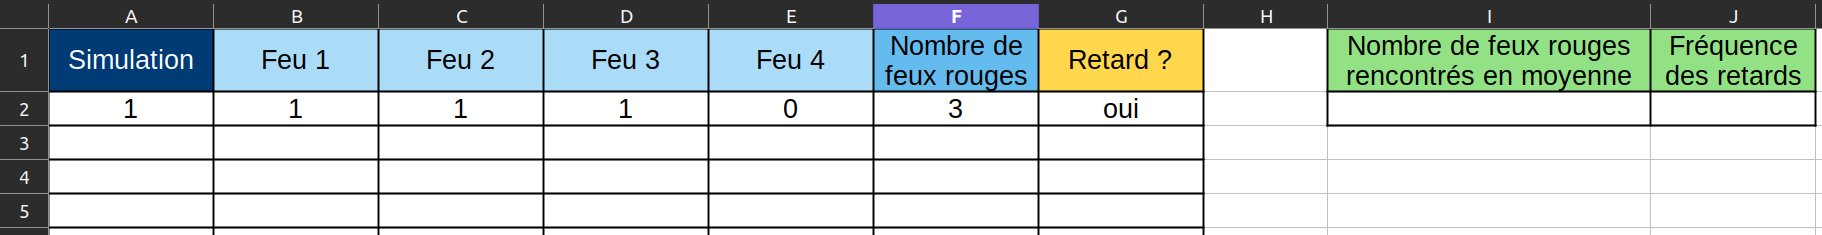
\includegraphics[width=0.9\linewidth]{Images/Tableur feux rouges.png}
	      \end{center}

	      \begin{enumerate}
		      \item Dans la cellule \texttt{B2}, saisir la formule \squared{\texttt{=SI(ALEA()<=2/3 ; 1 ; 0)}}. Quel(s) résultat(s) renvoie cette fonction, et avec quelle probabilité ? \correctionDots{Elle renvoie $1$ avec probabilité $2/3$, et $0$ avec probabilité $1/3$.}

		            Copier la formule dans les cellules \texttt{C2}, \texttt{D2} et \texttt{E2}.
		      \item Compléter la cellule \texttt{F2} en utilisant la fonction \texttt{SOMME}.
		      \item Compléter la cellule \texttt{G2} en utilisant la fonction \texttt{SI}.
		      \item Copier les cellules afin de réaliser $500$ simulations.
		      \item Compléter la cellule \texttt{I2}. Quel semble être le nombre moyen de feux rencontrés ? \correctionDots{$≈2,6$}
	      \end{enumerate}
	\item On peut utiliser la touche \texttt{F9} pour réaliser $500$ nouvelles simulations.

	      En complétant la cellule \texttt{J2}, peut-on répondre à la question de l'énoncé ?
\end{enumerate}

\tipbox{
	{\large\uline{AIDE TABLEUR}}

	\begin{itemize}
		\item \texttt{=SI(test ; "affichage 1" ; "affichage 2")} renvoie l'affichage 1 si le test est vrai, et l'affichage 2 si le test est faux.
		\item \texttt{=SOMME(A1;A5)} renvoie \texttt{A1 + A5}.
		\item \texttt{=SOMME(A1:A5)} renvoie \texttt{A1 + A2 + A3 + A4 + A5}.
		\item La fonction \squared{\texttt{=NB.SI(A1:A12 ; 5)}} renvoie le nombre de cellules comprises entre \texttt{A1} et \texttt{A12} dont le résultat est égal à $5$.
	\end{itemize}
}

\end{document}